\begin{exercise}
      {ID-25ad4aaf3aeaedcfea673f965c51157c659343f2}
      {Flächeninhalt}
  \ifproblem\problem
    Wie groß ist die graue Fläche?
    \begin{center}
      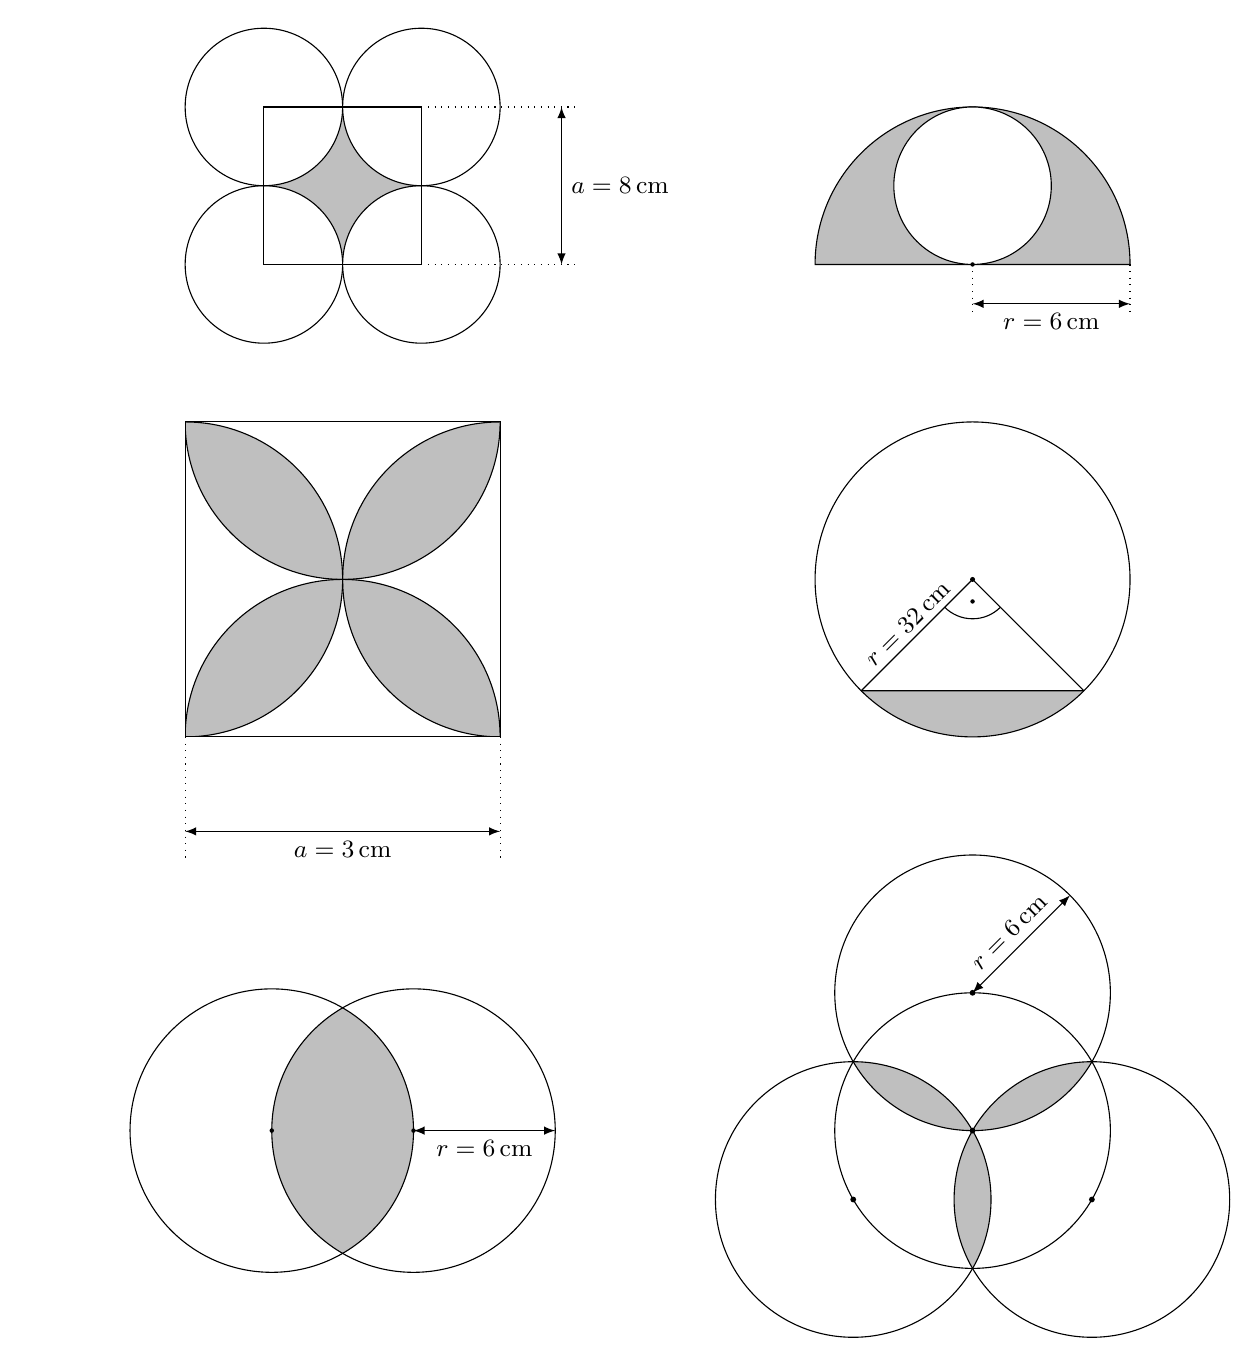
\begin{tikzpicture}
        % oberste Reihe
        \begin{scope}[scale=1]
          \filldraw[fill=white!75!black] (0, 0) rectangle (2, 2);
          \filldraw[fill=white] (0, 0) circle (1);
          \filldraw[fill=white] (2, 0) circle (1);
          \filldraw[fill=white] (0, 2) circle (1);
          \filldraw[fill=white] (2, 2) circle (1);
          \draw (0, 0) rectangle (2, 2);
          \draw[style=dotted] (2, 0) -- (4, 0);
          \draw[style=dotted] (2, 2) -- (4, 2);
          \draw[<->, >=latex] (3.78, 0) -- (3.78, 2);
          \node[right] at (3.78, 1) {{\small$a=8$\,cm}};
        \end{scope}
        \begin{scope}[scale=1, xshift=9cm, yshift=1cm]
          \filldraw[fill=white!75!black] (2, -1) arc (0:180:2) -- cycle;
          \filldraw[fill=white] (0, 0) circle (1);
          \fill (0, -1) circle (0.8pt);
          \draw[style=dotted] (0, -1) -- (0, -1.6);
          \draw[style=dotted] (2, -1) -- (2, -1.6);
          \draw[<->, >=latex] (0, -1.5) -- node[below] {{\small$r=6$\,cm}} (2, -1.5);
        \end{scope}
        % zweite Reihe
        \begin{scope}[xshift=-1cm, yshift=-6cm, scale=2]
          \begin{scope}
            \clip (0, 1) circle (1); % links
            \clip (1, 0) circle (1); % unten
            \fill[fill=white!75!black] (0, 0) rectangle (2, 2);
          \end{scope}
          \begin{scope}
            \clip (1, 0) circle (1); % unten
            \clip (2, 1) circle (1); % rechts
            \fill[fill=white!75!black] (0, 0) rectangle (2, 2);
          \end{scope}
          \begin{scope}
            \clip (2, 1) circle (1); % rechts
            \clip (1, 2) circle (1); % oben
            \fill[fill=white!75!black] (0, 0) rectangle (2, 2);
          \end{scope}
          \begin{scope}
            \clip (0, 1) circle (1); % links
            \clip (1, 2) circle (1); % oben
            \fill[fill=white!75!black] (0, 0) rectangle (2, 2);
          \end{scope}
          \begin{scope}
            \clip (0, 0) rectangle (2, 2);
            \draw (0, 1) circle (1); % links
            \draw (1, 0) circle (1); % unten
            \draw (2, 1) circle (1); % rechts
            \draw (1, 2) circle (1); % oben
          \end{scope}
          \draw (0, 0) rectangle (2, 2);
          \draw[style=dotted] (0, 0) -- (0, -0.8);
          \draw[style=dotted] (2, 0) -- (2, -0.8);
          \draw[<->, >=latex] (0, -0.6) -- node[below] (1, 0) {{\small$a=3$\,cm}} (2, -0.6);
        \end{scope}
        \begin{scope}[xshift=9cm, yshift=-4cm, scale=1]
          \begin{scope}
            \clip (0, 0) circle (2);
            \clip (225:2) -- ++(315:2) -- ++(45:2) -- ++(135:2) -- cycle;
            \fill[fill=white!75!black] (0, 0) circle (2);
          \end{scope}
          \draw (0, 0) circle (2);
          \filldraw[fill=white, join=bevel] (0, 0) -- (225:2) -- (315:2) -- cycle;
          \fill (0, 0) circle (0.9pt);
          \begin{scope}
            \clip (0, 0) -- (225:2) -- (315:2) -- cycle;
            \draw (0, 0) circle (0.5);
            \fill (270:0.28) circle (0.8pt);
          \end{scope}
          \node[rotate=45, above=-6pt] at (215:1) {{\small$r=32$\,cm}};
        \end{scope}
        % dritte Reihe
        \begin{scope}[xshift=1cm, yshift=-11cm, scale=0.9]
          \begin{scope}
            \clip (-1, 0) circle (2);
            \clip ( 1, 0) circle (2);
            \fill[fill=white!75!black] (0, 0) circle (2);
          \end{scope}
          \draw (-1, 0) circle (2);
          \draw ( 1, 0) circle (2);
          \fill ( 1, 0) circle (0.9pt);
          \fill (-1, 0) circle (0.9pt);
          \draw[<->, >=latex] (1, 0) -- node[below] {{\small$r=6$\,cm}} (3, 0);
        \end{scope}
        \begin{scope}[xshift=9cm, yshift=-11cm, scale=1.75]
          \begin{scope}
            \clip ( 90:1) circle (1);
            \clip (210:1) circle (1);
            \fill[fill=white!75!black] (0 , 0) circle (1);
          \end{scope}
          \begin{scope}
            \clip (210:1) circle (1);
            \clip (330:1) circle (1);
            \fill[fill=white!75!black] (0 , 0) circle (1);
          \end{scope}
          \begin{scope}
            \clip ( 90:1) circle (1);
            \clip (330:1) circle (1);
            \fill[fill=white!75!black] (0 , 0) circle (1);
          \end{scope}
          \draw (0 , 0) circle (1);
          \draw ( 90:1) circle (1);
          \draw (210:1) circle (1);
          \draw (330:1) circle (1);
          \fill (0 , 0) circle (0.6pt);
          \fill ( 90:1) circle (0.6pt);
          \fill (210:1) circle (0.6pt);
          \fill (330:1) circle (0.6pt);
          \draw[<->, >=latex] (90:1) -- node[rotate=45, above] {{\small$r=6$\,cm}} ++(45:1);
        \end{scope}
      \end{tikzpicture}
    \end{center}
  \fi
  %\ifoutline\outline
  %\fi
  %\ifoutcome\outcome
  %\fi
\end{exercise}
